%____________________________________________________________________________||
%FIXME: undefined reference to new systematic section
\section{Corrections to cross section for SM samples}
\label{sec:sideband_corrections}

The cross sections for the most relevant SM background are summarised in Table~\ref{tab:cross_sections_bkg}.

\begin{table}[!h]
  \scriptsize
  \centering
  \topcaption{Cross sections for the main SM backgrounds.}
  \label{tab:cross_sections_bkg}
  \begin{tabular}
    {c|c|c|c}
    \hline\hline
    \textbf{Sample} & \textbf{Cross section (pb)} & \textbf{Accuracy} & \textbf{K-factor} \\
    \hline
    W+jets, $100 < \scalht < 200$ GeV & $1347 \pm 2$ & LO & 1.21 \\
    W+jets, $200 < \scalht < 400$ GeV & $360 \pm 1$ & LO & 1.21 \\
    W+jets, $400 < \scalht < 600$ GeV & $48.9 \pm 0.17$ & LO & 1.21 \\
    W+jets, $600 < \scalht < 800$ GeV & $12.8 \pm 0.4$ & LO & 1.21 \\
    W+jets, $800 < \scalht < 1200$ GeV & $5.26 \pm 0.19$ & LO & 1.21 \\
    W+jets, $1200 < \scalht < 2500$ GeV & $1.33 \pm 0.05$ & LO & 1.21 \\
    W+jets, $\scalht > 2500$ GeV & $0.0309 \pm 0.0011$ & LO & 1.21 \\
    \hline
    DY+jets, $100 < \scalht < 200$ GeV & $139 \pm 4$ & LO & 1.23 \\
    DY+jets, $200 < \scalht < 400$ GeV & $42.8 \pm 1.4$ & LO & 1.23 \\
    DY+jets, $400 < \scalht < 600$ GeV & $5.5 \pm 0.2$ & LO & 1.23 \\
    DY+jets, $\scalht > 600$ GeV & $2.2 \pm 0.8$ & LO & 1.23 \\
    \hline
    \gj, $40 < \scalht < 100$ GeV & $20730 \pm 66$ & LO & - \\
    \gj, $100 < \scalht < 200$ GeV & $9226 \pm 36$ & LO & - \\
    \gj, $200 < \scalht < 400$ GeV & $2281 \pm 47$ & LO & - \\
    \gj, $400 < \scalht < 600$ GeV & $273 \pm 9$ & LO & - \\
    \gj, $\scalht > 600$ GeV & $94.5 \pm 3.2$ & LO & - \\
    \hline
    $Z\rightarrow \nu\nu$+jets, $100 < \scalht < 200$ GeV & $280.47$ & LO & 1.23 \\
    $Z\rightarrow \nu\nu$+jets, $200 < \scalht < 400$ GeV & $78.36$ & LO & 1.23 \\
    $Z\rightarrow \nu\nu$+jets, $400 < \scalht < 600$ GeV & $10.94$ & LO & 1.23 \\
    $Z\rightarrow \nu\nu$+jets, $\scalht > 600$ GeV & $4.20$ & LO & 1.23 \\
    \hline
    TTJets & $831.76^{+20}_{-30}$ & NNLO & - \\    
    \hline \hline
  \end{tabular}
\end{table}

In the high-\scalht, high-\etmiss corner of the phase space used in this search, the normalisations of the MC samples do not necessarily agree with the observation. 
Moreover, the cross section is known only to a limited number of perturbative orders and additional corrections could be in principle sizeable. \\
The analysis strategy for the background predictions is built in such a way to be mildly, if not negligibly, dependent on these corrections. 
The backgrounds are estimated from control regions in data, and the effect of cross section corrections on the transfer factors is expected to largely cancel out, 
because the background composition is very similar between the signal region and the control regions used to estimate each background. \\
However, the ``data-driven'' tests described in Sec.~\ref{sec:closure-tests} would benefit from a better control of the normalisation of MC samples, 
since more aggressive extrapolations are carried on there with respect to the background predictions in the analysis. 
As an example, the $0 \rightarrow 1$ b-tag test carried on in the single muon control sample, utilises 
a $W$-enriched sample to predict a $t\bar{t}$-enriched one and is thus sensitive to the relative corrections of $W$ with respect to $t\bar{t}$. 
In this perspective, the systematics derived with the data-driven tests can improve 
by measuring residual cross section corrections to the main background processes using the data. \\
In the previous iteration of the analysis, this was done using sidebands 
in the control regions enriched in a specific process (see Sec.~\ref{app:sideband-corrections-old} for more details). 
For this analysis, the full phase-space of the sideband is considered, 
and corrections are extracted from a maximum likelihood fit, as described in Sec.~\ref{sec:fit-sideband}. \\
The sideband corrections are derived after all the other corrections to the MC and data are applied, 
such as trigger efficiency, data/MC scale factors (b-tag, lepton ID/isolation, etc.) and jet energy scale. 
The sideband corrections are applied and propagated to all the steps of the analysis.\\
No uncertainty is considered for these corrections as any inaccuracy is already accounted 
for in the data-driven tests described in Sec.~\ref{sec:closure-tests} and would result in inflated systematics. 

\textbf{As the understanding of the new data is still in a preliminary stage and some crucial corrections to the MC 
are not yet in place, for the moment the corrections derived in 2015, described in Sec.~\ref{app:sideband-corrections-old} and listed in Tab.~\ref{tab:sbCorrs}, are used in the analysis. }

The section is organised as follow. 
In Sec.~\ref{sec:bias-study-sideband} the sidebands taken for each process are described and variations of known sources of 
systematic uncertainty are used to study potential bias. In Sec.~\ref{sec:fit-sideband} the procedure used for deriving
the corrections is described and the corrections derived with this study are summarised in Table~\ref{tab:sbCorrsFromFit}.\\
In Sec.~\ref{app:sideband-corrections-old} is a comparison 
between the corrections derived for the old and new methods using the 2015 data.

\subsection{Definition of sidebands and study of bias}
\label{sec:bias-study-sideband}
\subsubsection{\gj sideband}
The cross section used for this process is at LO accuracy and no $k$-factor is applied. 
As a result, some disagreement between data and MC is expected in the single photon control region.
The observation confirms indeed this hypothesis, with the simulation underestimating the yields by $\sim 20\%$. \\
A correction is derived using a sideband in data by inverting the \alphat cut. 
For $400 < \scalht < 600$ GeV, events are selected in the interval $0.50 < \alphat < 0.52$, 
while for $600 \leq \scalht < 800$ GeV the sideband is defined by the cut $0.50 < \alphat < 0.53$. \\
To understand the effect of known systematic sources the ratio of the proportional change in the
predicted sideband yield after the systematic variation over the change in the control region yield is shown in 
Fig.~\ref{fig:pho-bias-sideband} (the separate shifts for control and sideband regions are shown in
App.~\ref{app:prop-shift-syst} )
The bias in the sideband under these variations is seen to be
subdominant compared to the statistical uncertainty of the sample.
Any residual bias is accounted for by including these systematics 
in the fit when when deriving the sideband corrections.

\begin{figure}[!h]
  \centering
    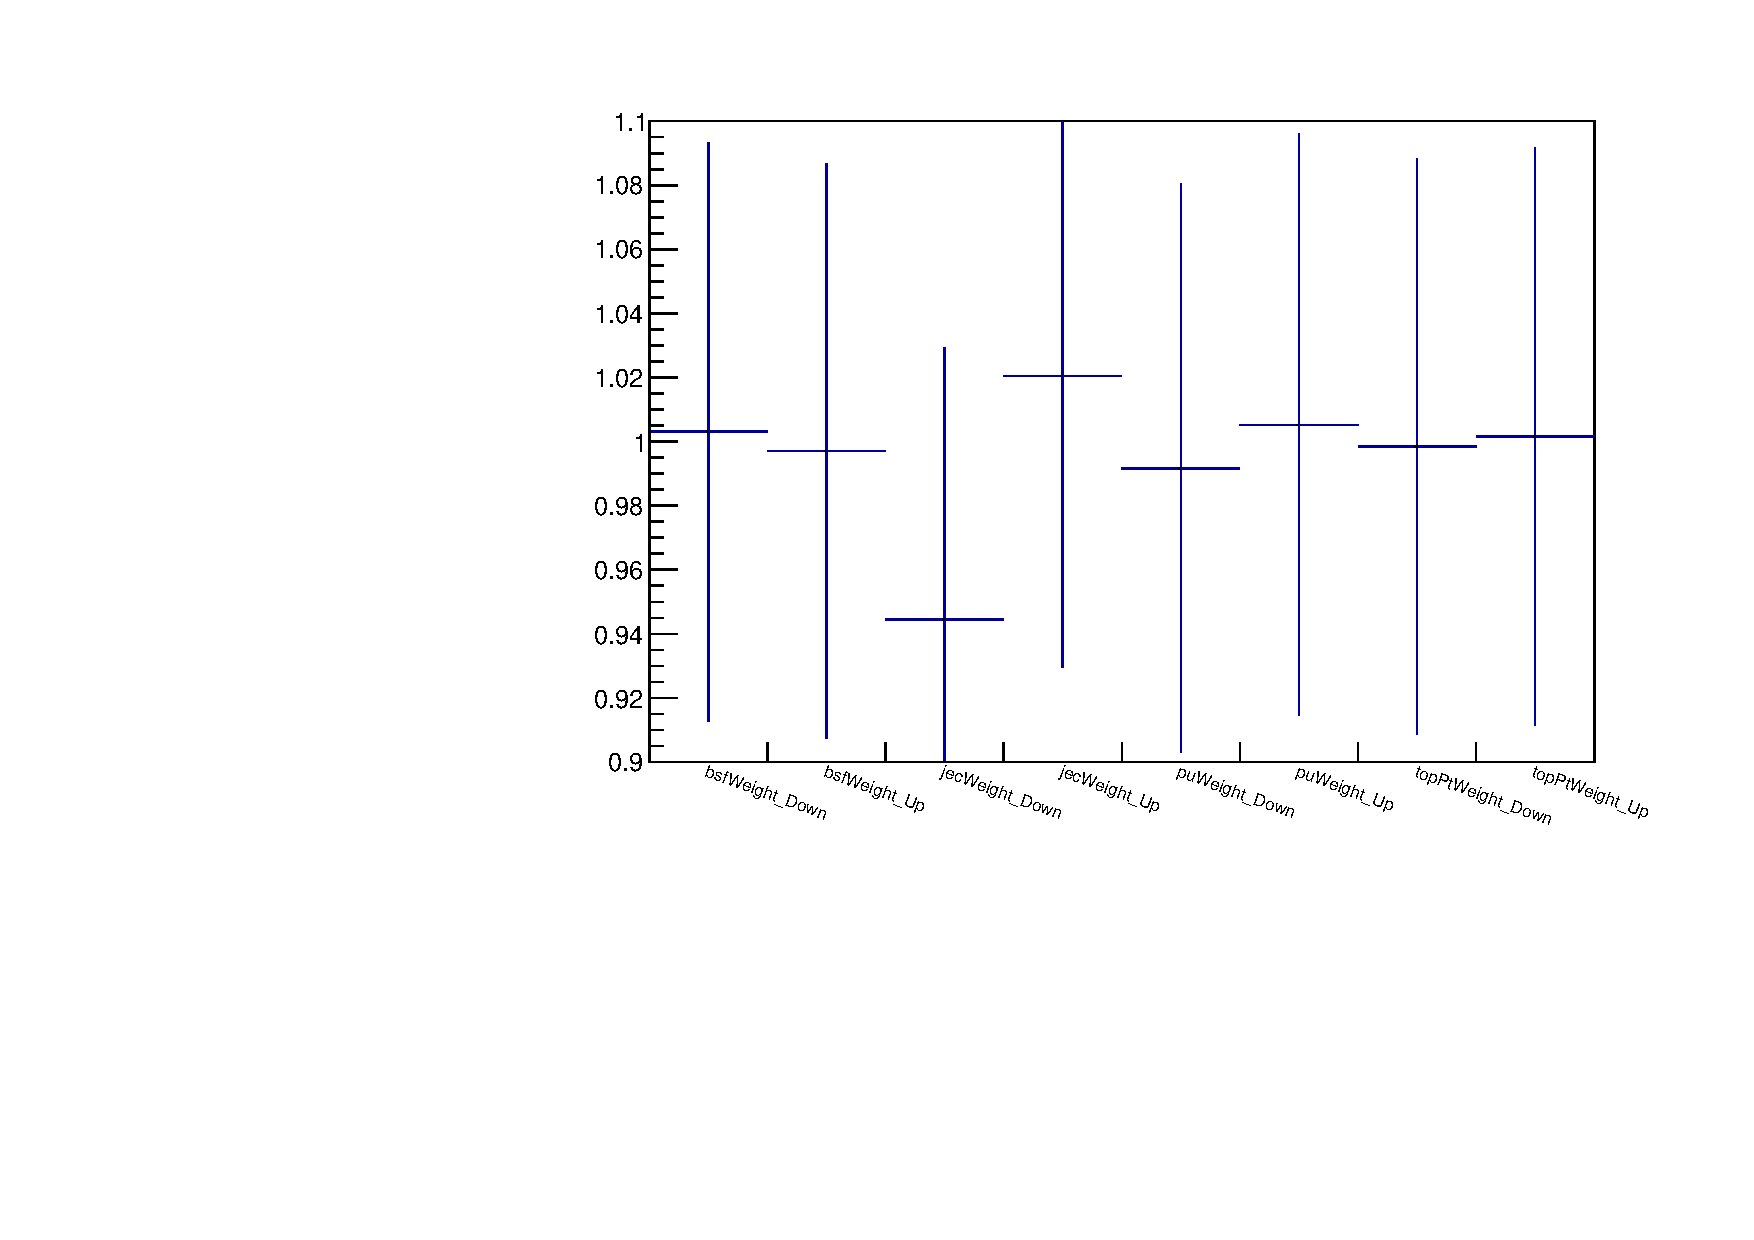
\includegraphics[width=0.9\textwidth]{figures/sideband_fit/summary_MhtSB_SinglePhoton.pdf}
  }~~
  \caption{Double ratio for \gj of change in MC yield under variations of known systematic sources in the sideband to the control region.
  The error bars represent the statistical uncertainty in the sideband and control region. No large biases (significantly higher than the statistical power of the sample) are observed.}
  \label{fig:pho-bias-sideband}
\end{figure}

\subsubsection{\mj and \mmj sideband}
For the $W$+jets, \ttbar+jets and $Z$+jets samples the cross section is know with better accuracy with respect to the \gj process, 
with NLO QCD or better precision.
However, some inconsinstency could arise from the different cross section calculations, since for \wj and \zj the LO cross sections 
are corrected with NLO k-factor (1.21 and 1.23 respectively) while for \ttbar the full NNLO calculation is used. \\
The corrections for these processes are derived using a sideband defined by inverting the \mht cut, namely 
applying the selection $100 < \mht < 130$ GeV. \\
As for the \gj sidebands, the change in the ratio of MC yields in the sideband
to the yields in the control region after the variation of several sources of systematic uncertainty is shown in 
Fig.~\ref{fig:mu-bias-sideband} and Fig.~\ref{fig:mumu-bias-sideband} (the separate shifts for control and sideband regions are shown in 
App.~\ref{app:prop-shift-syst}. This again shows that any
bias in the sideband with respect to the control regions for these systematic sources is 
subdominant compared to the statistical uncertainty of the sample (shown in the error bars).
Any residual bias is accounted for by including these systematics 
in the fit when when deriving the sideband corrections.


\begin{figure}[!h]
  \centering
    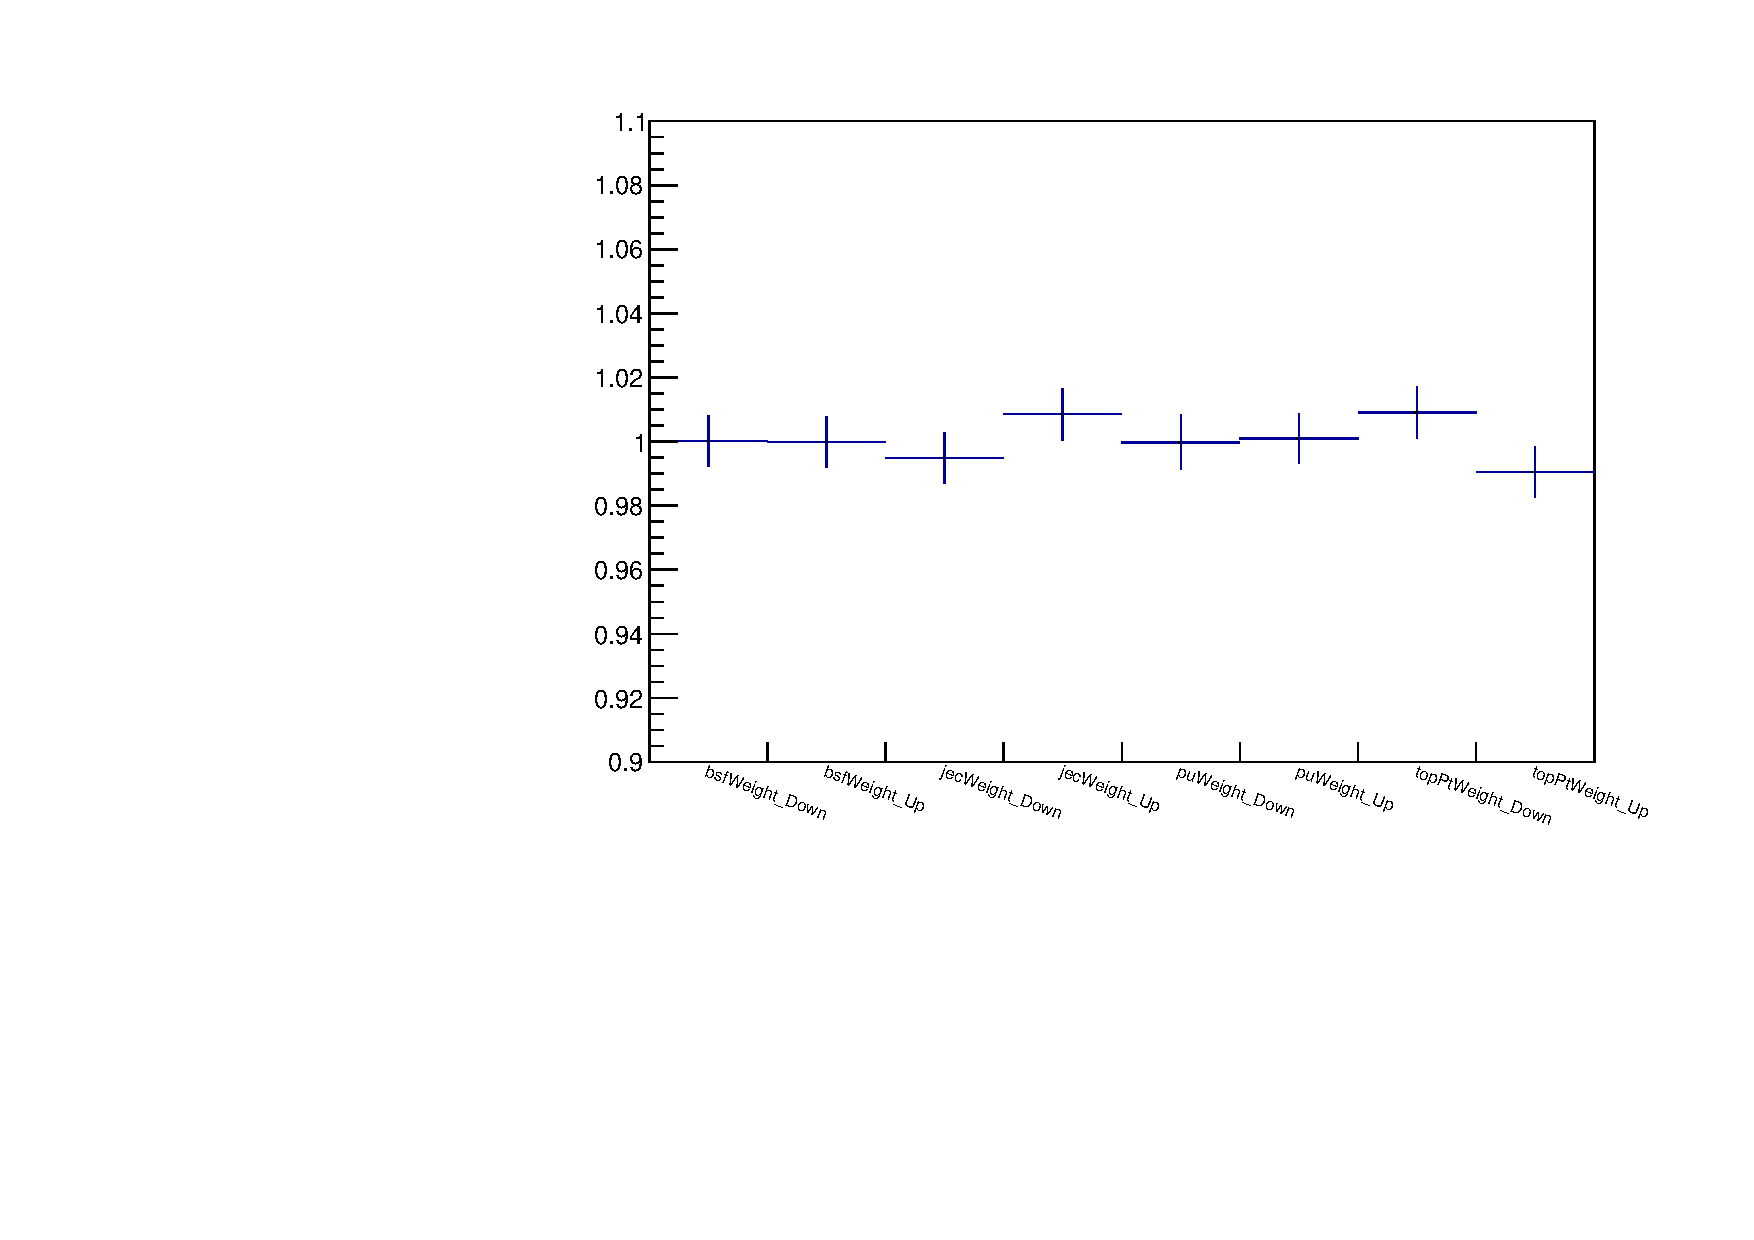
\includegraphics[width=0.9\textwidth]{figures/sideband_fit/summary_MhtSB_SingleMu.pdf}
  }~~
  \caption{Double ratio for \mj of change in MC yield under variations of known systematic sources in the sideband to the control region.
  The error bars represent the statistical uncertainty in the sideband and control region. No large biases (significantly higher than the statistical power of the sample) are observed.}
  \label{fig:mu-bias-sideband}
\end{figure}

\begin{figure}[!h]
  \centering
    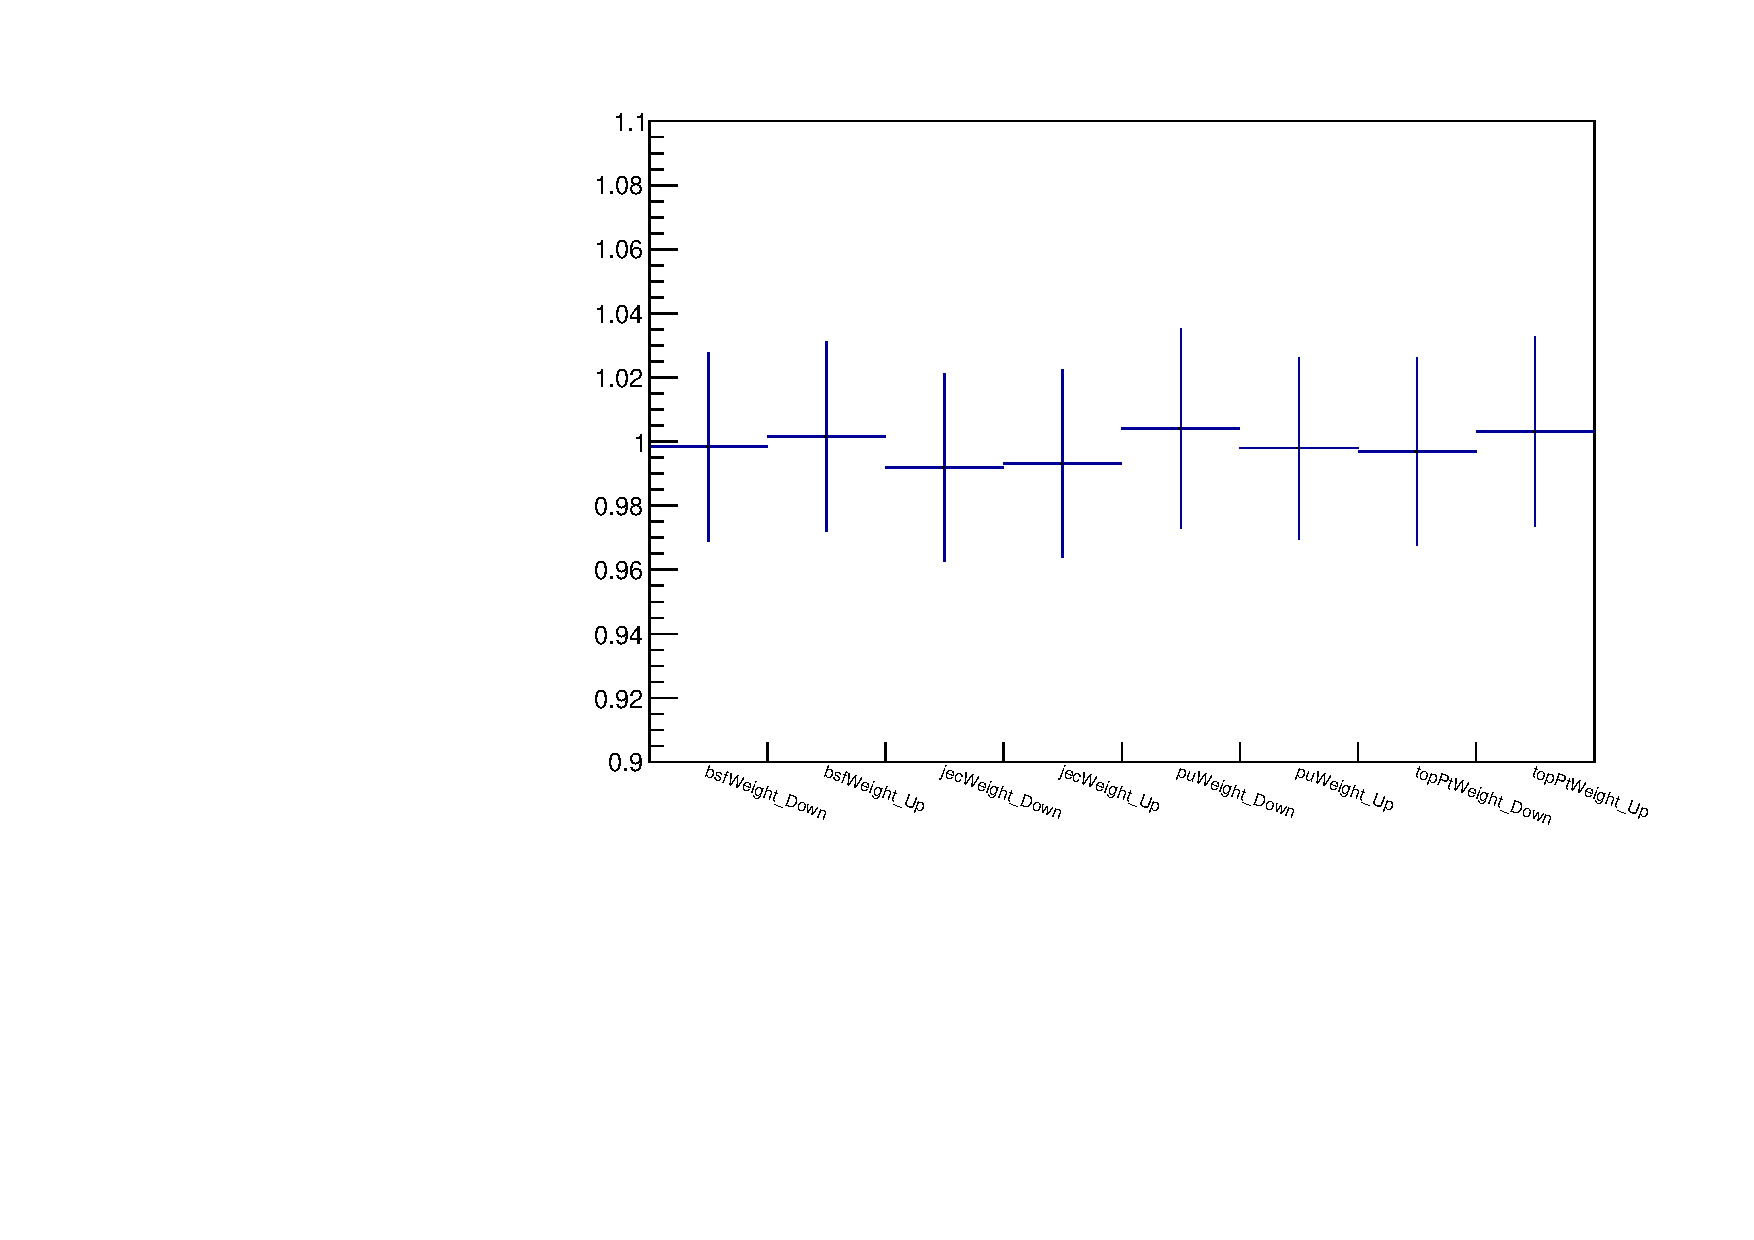
\includegraphics[width=0.9\textwidth]{figures/sideband_fit/summary_MhtSB_DoubleMu.pdf}
  }~~
  \caption{Double ratio for \mmj of change in MC yield under variations of known systematic sources in the sideband to the control region.
  The error bars represent the statistical uncertainty in the sideband and control region. No large biases (significantly higher than the statistical power of the sample) are observed.}
  \label{fig:mumu-bias-sideband}
\end{figure}
\subsection{Procedure for deriving sideband corrections}
\label{sec:fit-sideband}

To take advantage of the full phase space of the sidebands a simultaneous 
fit is used to derive the corrections for \wj, \zj, \ttbar and \gj. 
The sideband is binned identically to the control region in \njet, \nb and \scalht and a floating 
parameter per relevant process encodes the correction for that process (fully correlated across all bins).
The \wj and \ttbar processes are mainly constrained by the \mj sideband while the \zj and \gj processes are
wholey constrained by the \mmj and \gj sidebands respectively. The values of the corrections and uncertainties
given by the fit are shown in Table~\ref{tab:sbCorrsFromFit}.

\begin{table}[!h]
  \scriptsize
  \centering
  \topcaption{Cross section corrections for SM backgrounds derived with fit to sidebands in data.}
  \label{tab:sbCorrsFromFit}
  \begin{tabular}
    {cllc}
    \hline\hline
    \textbf{Process} & \textbf{Sideband} & \textbf{Selection} & \textbf{Corrrection} \\
    \hline
    \gj & $0.50 < \alphat < 0.52(0.53)$ & \gj & $1.43 \pm 0.07$ \\
    \wj & $100 < \mht < 130 \, \mathrm{GeV}$ & \mj& $1.23 \pm 0.02$ \\
    \zj & $100 < \mht < 130 \, \mathrm{GeV}$ & \mmj& $1.14 \pm 0.05$ \\
    \ttbar + jets & $100 < \mht < 130 \, \mathrm{GeV}$ & \mj, \mmj  & $0.9 \pm 0.02$ \\
    \hline \hline
  \end{tabular}
\end{table}
